\textit{This part of the thesis covers the RQ1 and is one of the Semantic Web foundations, which is the possibility to dereference URIs to let applications negotiate their semantic content.
However, this exploitation is often infeasible as the availability of such information depends on the reliability of networks, services, and human factors.
Moreover, it has been shown that around 90\% of the information published as Linked Open Data is available as data dumps and more than 60\% of endpoints are offline.
To this end, we propose a Web service called \textit{Where is my URI?}.
Our service aims at indexing URIs and their use in order to let Linked Data consumers find the respective RDF data source, in case such information cannot be retrieved from the URI alone.
We rank the corresponding datasets by following the rationale upon which a dataset contributes to the definition of a URI proportionally to the number of literals.
We finally describe potential use-cases of applications that can immediately benefit from our simple yet useful service.}

\subsection{The WIMU approach}
%\todo[inline]{Saleem: I wrote a new introduction highlighted in blue. Of course this still needs further polishing. }
In the Web of Data, applications such as Link Discovery or Data Integration frameworks need to know where a specific URI is located.
However, due to decentralized architecture of the Web of data, reliability and availability of Linked Data services, locating such URIs is not a trivial task.
Locating the URIs from a well-known data dump might be easy. 
For example, it is trivial to know that the URI \url{http://dbpedia.org/resource/Leipzig} belongs to the DBpedia dataset. 
However, locating the dataset where the URI \url{http://citeseer.rkbexplorer.com/id/resource-CS116606} was first defined is a time-consuming task. 
Consequently, this can greatly affect the scalable and time-efficient deployment of many Semantic Web applications such as link discovery, Linked Data enrichment, and federated query processing.
On the other hand, such provenance information about URIs can lead to regenerate and validate the links across datasets.

The availability of the current available services to provide such information is unfortunately one of the key issues in Semantic Web and Linked Data.
It has been shown that around 90\% of the information published as Linked Open Data is available as data dumps only and more than 60\% of endpoints are offline \cite{vandenbussche2017sparqles}.
The availability problem is mostly due to cost associated with storing and providing querying services.%\todo{Maybe write something more here about the how much URIs are actually dereferenceable.}

To this end, we propose \textit{Where is my URI?} \ac{WIMU}, a low-cost Semantic Web service to determine the RDF data source of URIs along with their use. 
We also rank the data sources in case a single URI is provided by multiple data sources. The ranking is based-on a scoring function. 
Currently, our service processed more than 58 billion unique triples from more than 660,000 datasets obtained from LODStats~\cite{auer2012lodstats} and LOD Laundromat~\cite{beek2014lod}. 
For each URI, our service provides the corresponding datasets and the number of literals in the datasets having this URI. 
The service is both available from a web interface as well as can be queried from a client application using the standard HTTP protocol. 
% The service provides the output as JSON-LD, a JSON-based W3C standard for the serialization of Linked Data. 
We believe our service can be used in multiple Linked Data related problems such as devising fast link discovery frameworks, efficient source selection, and distributed query processing.

Our main contributions are as follows:
\begin{itemize}
    \item We provide a regularly updated\footnote{Updated monthly due to the huge size of data processed.} database index of more than 660K datasets from LODStats and LOD Laundromat. 
    \item We provide an efficient, low cost and scalable service on the web that shows which dataset most likely defines a URI. 
    \item We provide various statistics of datasets indexed from LODStats and LOD Laundromat.
\end{itemize}
The service is available from \url{https://wimu.aksw.org/} under GNU Affero public license 3.0 and the source code is available online\footnote{Link to the GitHub repository: \url{https://github.com/dice-group/wimu}}.

The rest of the chapter is organized as follows: 
We discuss the proposed approach in detail, including the index creation, the web interface, and the data processing. 
We finally present our evaluation results.

\subsection{The approach}

WIMU uses the number of literals as a heuristic to identify the dataset which most likely defines a URI.
The intuition behind this can be explained in two points: 
(1) Literal values are the raw data that can disambiguate a URI node in the most direct way and 
(2) The Semantic Web architecture expects that datasets reusing a URI only refer to it without defining more literal values. 
One more reason for point (1) is that: it is straightforward to understand whether two literal values are different, whereas disambiguating URIs usually requires more effort.

We store the collected data in an Apache Lucene\footnote{Link to the official web site: \url{https://lucene.apache.org/}} index.
Due to runtime performance and complexity reasons, we found that storing the information into Lucene was more convenient than a traditional triple store such as Virtuoso\footnote{Link to the official web site: \url{https://virtuoso.openlinksw.com/}}.
The rationale behind this choice is that a tuple such as \emph{(URI, Dataset, Score)} would be expressed using at least three triples; for instance:
\begin{verbatim}
:R001 :hasURI :URI001
:R001 :hasDataset :Dataset001
:R001 :hasScore "20"^^http://www.w3.org/2001/XMLSchema#Integer
\end{verbatim}
where \texttt{:R001} is an index record URI. Therefore, materializing all records would have substantially increased the space complexity of our index.

\subsubsection{The index creation}

\begin{figure}[htb] 
	\centering
	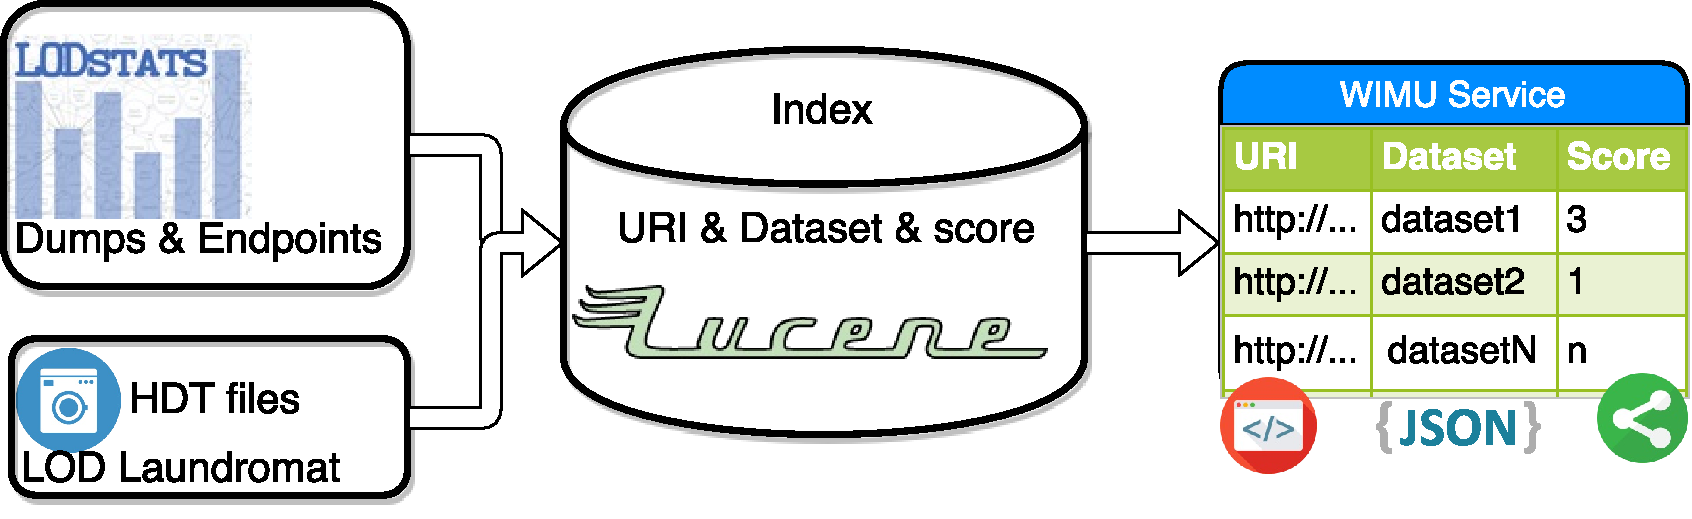
\includegraphics[width=250pt]{img/arq.pdf}
	\caption{Creation workflow of the WIMU index.}
	\label{fig:flow1}
\end{figure}

The index creation, the core of our work, is shown in figure \ref{fig:flow1} and consists in the following four steps:
\begin{enumerate}		
	\item Retrieve list of datasets from sources (i.e., LOD Stats and LOD Laundromat).
	\item Retrieve data from datasets (i.e., dump files, endpoints, and HDT files).
	\item Build three indexes from dump files, endpoints, and HDT files.
	\item Merge the indexes into one.
	\item Make the index available and browsable via a web application and an API service.
\end{enumerate}

For each processed dataset, we keep its URI as provenance.
After we have downloaded and extracted a dump file, we process it by counting the literals as objects for each subject.
For endpoints and HDT files, we use a SPARQL query:

\begin{verbatim}
   SELECT ?s (count(?o) as ?c) WHERE {
      ?s [] ?o . FILTER(isliteral(?o))  
   } GROUP BY ?s
\end{verbatim}

We process the data in parallel, distributing the datasets among the CPUs. 
If a dataset is too large for a CPU, we split it into smaller chunks.
To preserve space, dump files are deleted after being processed.
The index was generated using an Intel Xeon Core i7 processor with 64 cores, 128 GB RAM on an Ubuntu 14.04.5 LTS with Java SE Development Kit 8. %The results are available online.

\subsubsection{The web interface and the API service}

In order to simplify the access to our service, we create a web interface where it is possible to visualize all the data from the service, as figure \ref{fig:web} shows. 
% The web interface uses the service than the input and output are the same, the difference is that you can also visualize in a web browser, and if the user thinks that the URI were belongs to another dataset not listed, he can manually input a new dataset related to this URI, as the figure \ref{fig:web} presents.

\begin{figure}[htb] 
	\centering
	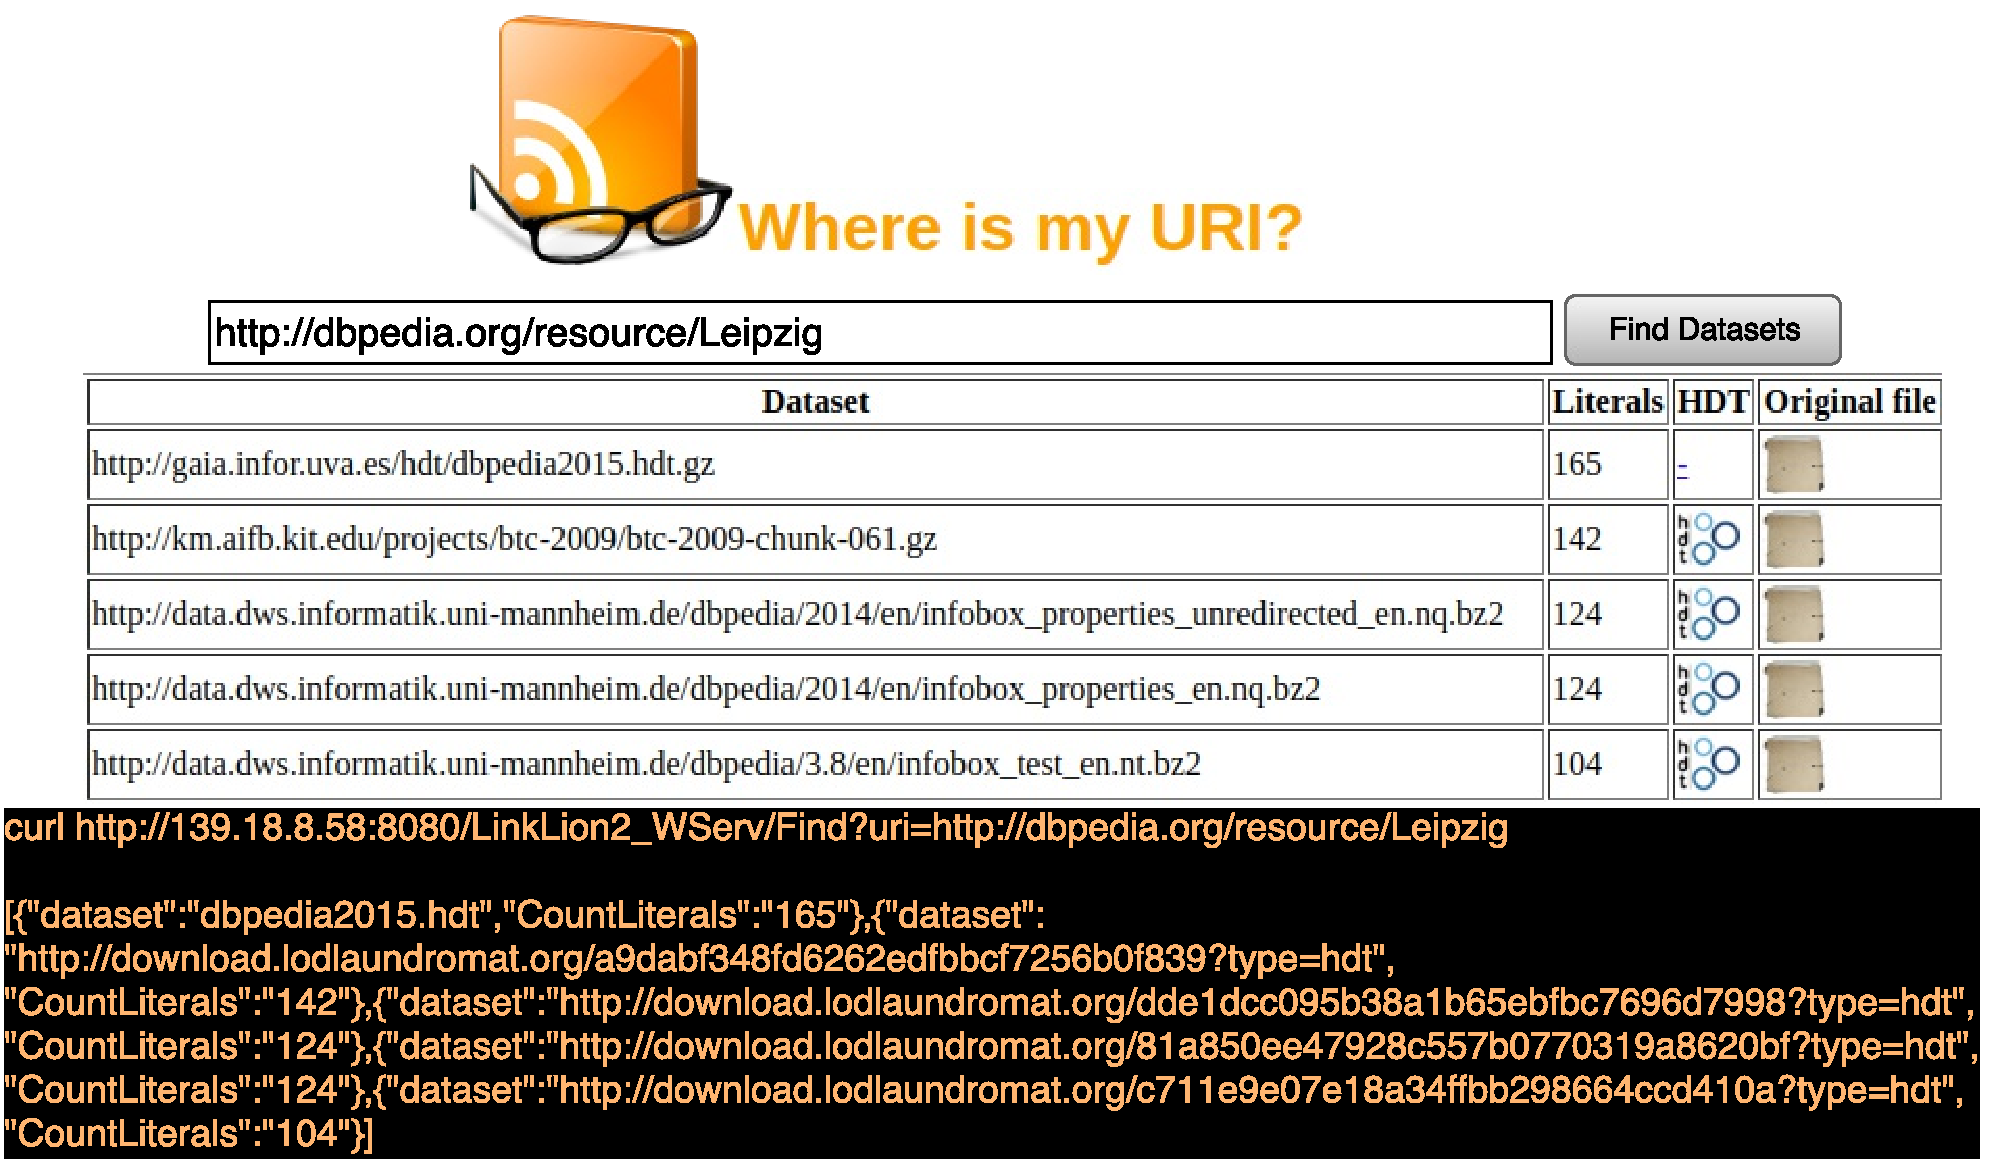
\includegraphics[width=350pt]{img/web.pdf}
	\caption{Web interface.}
	\label{fig:web}
\end{figure}

%The service has three types of input: a URI, a dataset URL or a SQL query, the output is in JSON-LD format. 
The web interface allows the user to query a URI and see the results in a HTML web browser; the API service allows the user to work with an output in JSON format. %, allowing them to use any programming language or platform that supports JSON format.
In figure \ref{fig:web}, we can see an example of usage of the service, where WIMU is requested for the dataset in which the URI \texttt{dbpedia:Leipzig} was defined.
%and the output are two datasets defining the URI, indicating that the dataset (\url{http://lov.okfn.org/dataset/lov/sparql}) most likely defines the URI because it's bigger number of literals.
figure \ref{fig:usage} shows the generic usage of WIMU.


\subsection{Use cases}

In this section, we present three use-cases to show that our hypothesis works on the proposed tasks.

\subsubsection{Data Quality in Link Repositories}

The first use-case is about quality assurance in a link repository by re-applying link discovery algorithms on the stored links.
This task concerns important steps of the Linked Data Lifecycle, in particular \textit{Data Interlinking} and \textit{Quality}.
Link repositories contain sets of links that connect resources belonging to different datasets. 
Unfortunately, the subject and the object URIs of a link often do not have metadata available, hence their Concise Bounded Descriptions (CBDs) are hard to obtain.
In following figure, $(D_1,...,D_n|x)$ : $D_n$ represent the datasets and $x$ is the quantity of literals. 
The \textbf{input} for our service in this use-case is $S$; the \textbf{output} is $\{(D_1,3),(D_2,1),(D_3,2)\}$, where $D1$ most likely defines $S$ due to the highest number of literal. 
In the same way, the dataset that most likely defines $T$ is $D_4$ with 7 literals. 
Once we have this information, the entire CBD of the two resources $S$ and $T$ can be extracted and a Link Discovery algorithm can check whether the \texttt{owl:sameAs} link among them should subsist.


\begin{figure}[htb] 
	\centering
	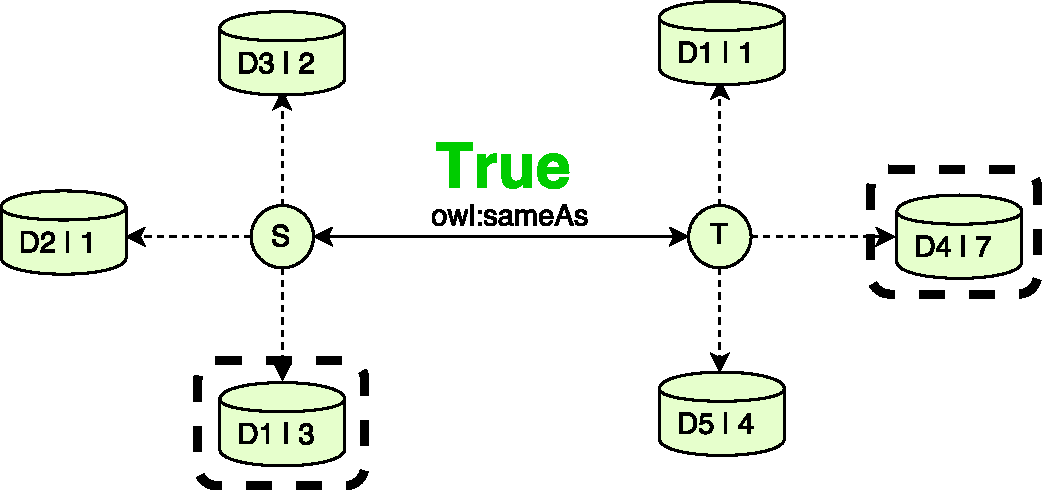
\includegraphics[width=250pt]{img/true.pdf}
	\label{fig:caseTrue}
	\caption{First use-case.}
\end{figure}

\subsubsection{Finding class axioms for Link Discovery}

A class axiom is needed by the link discovery algorithm to reduce the number of comparisons. 
Here, the aim is to find two class axioms for each mapping in the link repository.

To this end, we use real data including a mapping\footnote{Real data mapping from LinkLion: \url{http://www.linklion.org/download/mapping/citeseer.rkbexplorer.com---ibm.rkbexplorer.com.nt}} from the Link\-Lion repository~\cite{linklion2014} between \texttt{http://citeseer.rkbexplorer.com/id/resource-CS65161} ($S$) and \texttt{http://citeseer.rkbexplorer.com/id/resource-CS65161} ($T$). 
Our service shows that $S$ was defined in four datasets, whereas the dataset with more literals was \url{http://km.aifb.kit.edu/projects/btc-2009/btc-2009-chunk-039.gz}\footnote{Also available in HDT file from \url{http://download.lodlaundromat.org/15b06d92ae660ffdcff9690c3d6f5185?type=hdt}}. 
Thus, we can deduce where the URI $S$ was most likely defined.
Knowing the datasets allows us to extract the axioms of the classes our URIs belong to.
The techniques to decrease the complexity vary from choosing the most specific class to using an ontology learning tool such as DL-Learner~\cite{lehmann2009dl}.

\begin{figure}[htb] 
	\centering
	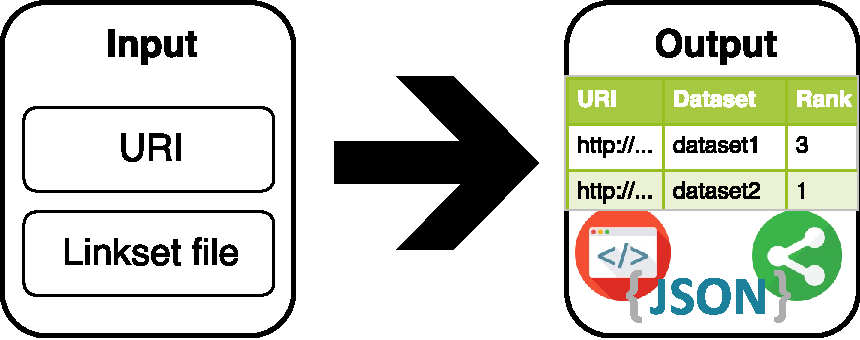
\includegraphics[width=150pt]{img/usage.pdf}
	\caption{Usage.}
	\label{fig:usage}
\end{figure}

\subsubsection{Federated Query Processing}
Federated queries, which aim to collect information from more than one datasets is of central importance for many semantic web and linked data applications~\cite{saleem2013fostering,bigtcga2014}. One of the key step in federated query processing is the \emph{source selection}. The goal of the source selection is to find relevant sources (i.e., datasets) for the given user query. In the next step, the federated query processing engine makes use of the source selection information to generate an optimized query execution plan. WIMU can be used by the federated SPARQL engines to find the relevant sources against the individual triple patterns of the given SPARQL query. In particular, our service can be helpful during the source selection and query planning in cost-based SPARQL federation engines such SPLENDID~\cite{splendid2011}, SemaGrow~\cite{semagrow2015}, HiBISCuS~\cite{hibiscus2014}, CostFed~\cite{costfed2017}, etc.  

\subsubsection{Usage examples}
The service API provides a JSON as output, allowing users to use WIMU with some programming language compatible with JSON.
Here we give examples, for more details please check the manual\footnote{More examples such as many URIs, linksets, and generation of Concise Bounded Description (CBD) check \url{https://dice-group.github.io/wimu/}}.

\textbf{Service}: \url{https://wimu.aksw.org/Find}

Parameters table \ref{tab:param}:
% Please add the following required packages to your document preamble:
% \usepackage{booktabs}
\begin{table}[]
\centering
\caption{Parameters}
\label{tab:param}
\resizebox{\textwidth}{!}{
\begin{tabular}{@{}lll@{}}
\toprule
\textbf{Parameter} & \textbf{Default} & \textbf{Description}                                      \\ \midrule
top                & 0                & Top ocurrences of the datasets where the URI was defined. \\
uri                & -                & URI expected to search .                                  \\ \bottomrule
\end{tabular}}
\end{table}

Input (Single URI example): 

\url{https://wimu.aksw.org/Find?top=5&uri=http://dbpedia.org/resource/Leipzig}

Output:
\begin{lstlisting}[language=JSON]
[
 {
  "dataset": 
  "http://downloads.dbpedia.org/2016-10/core-i18n/en/infobox_properties_en.ttl.bz2",
  "CountLiteral": "236"
 },
 {
  "dataset": "http://gaia.infor.uva.es/hdt/dbpedia2015.hdt.gz",
  "CountLiteral": "165"
 },
 {
  "dataset": 
  "http://download.lodlaundromat.org/a9dabf348fd6262edfbbcf7256b0f839?type=hdt",
  "CountLiteral": "142"
 },
 {
  "dataset": 
  "http://download.lodlaundromat.org/dde1dcc095b38a1b65ebfbc7696d7998?type=hdt",
  "CountLiteral": "124"
 }
]
\end{lstlisting}

Java and the API Gson\footnote{Link to the official web site: \url{https://github.com/google/gson}}:
\begin{lstlisting}[language=JAVA]
private void exampleJson() throws Exception {
  String service = "https://wimu.aksw.org/Find?uri=";
  String uri = "http://dbpedia.org/resource/Leipzig";
  URL url = new URL(service + uri);
  InputStreamReader reader = new InputStreamReader(url.openStream());
  WIMUDataset wData = new Gson().fromJson(reader, WIMUDataset[].class)[0];
  System.out.println("Dataset:" + wData.getDataset());
  System.out.println("Dataset(HDT):" + wData.getHdt());
}
\end{lstlisting}


\subsection{Evaluation: Statistics about the Datasets}\label{ev:wimu}

% SPARQLES is the only monitoring endpoints~\cite{vandenbussche2017sparqles}

To the best of our knowledge, LODStats\cite{auer2012lodstats} is the only project oriented to monitoring dump files; however, its last update dates back to 2016. 
Observing table \ref{tab:lodstats}, we are able to say that from LODStats, not all datasets are ready to use.
Especially, more than 58\% are off-line, 14\% are empty datasets, 8\% of the triples that have literals as objects are blank nodes and 35\% of the online datasets present some error using the Apache Jena parser\footnote{See \url{https://github.com/dice-group/wimu/blob/master/ErrorJenaParser.tsv}.}. 
A large part of those data was processed and cleaned by LOD Laundromat~\cite{beek2014lod}.


\setlength{\tabcolsep}{0.5em} % for the horizontal padding
\begin{table}[H]
	\centering
	\caption{Datasets.}
	\label{tab:lodstats}
	\resizebox{\textwidth}{!}{
    \begin{tabular}{lrrr}
    \toprule
    & \textbf{LOD Laundromat} & \textbf{LODStats} & \textbf{Total} \\ 
    \midrule
    \textbf{URIs indexed} & 4,185,133,445 & 31,121,342 & 4,216,254,787 \\
    \textbf{Datasets checked} & 658,206 & 9,960 & 668,166 \\
    \textbf{Triples processed} & 19,891,702,202 & 38,606,408,854 & 58,498,111,056 \\
    \bottomrule
    \end{tabular}}
\end{table}

The algorithm took three days and seven hours to complete the task. 
Thus, we will create a scheduled job to update our database index once a month.
With respect to the information present in the figure \ref{fig:dumps}, we can observe that the majority of files from LODStats are in RDF/XML format.
Moreover, the endpoints are represented in greater numbers (78.6\%), the dominant file format is RDF with 84.1\% of the cases, and 56.2\% of errors occurred because Apache Jena was not able to perform SPARQL queries.
Among the HDT files from LOD Laundromat, 2.3\% of them could not be processed due to parsing errors.
Another relevant point is that 99.2\% of the URIs indexed with WIMU come from LOD Laundromat, due to 69.8\% of datasets from LODstats contain parser errors in which WIMU was not able to process the data.
%https://docs.google.com/spreadsheets/d/15kh8E4WllXG5Xdp1aL-JiHvnXAiVC6a8XqVUJ1gtMZ8/edit?usp=sharing

\begin{figure}[htp] 
	\centering
	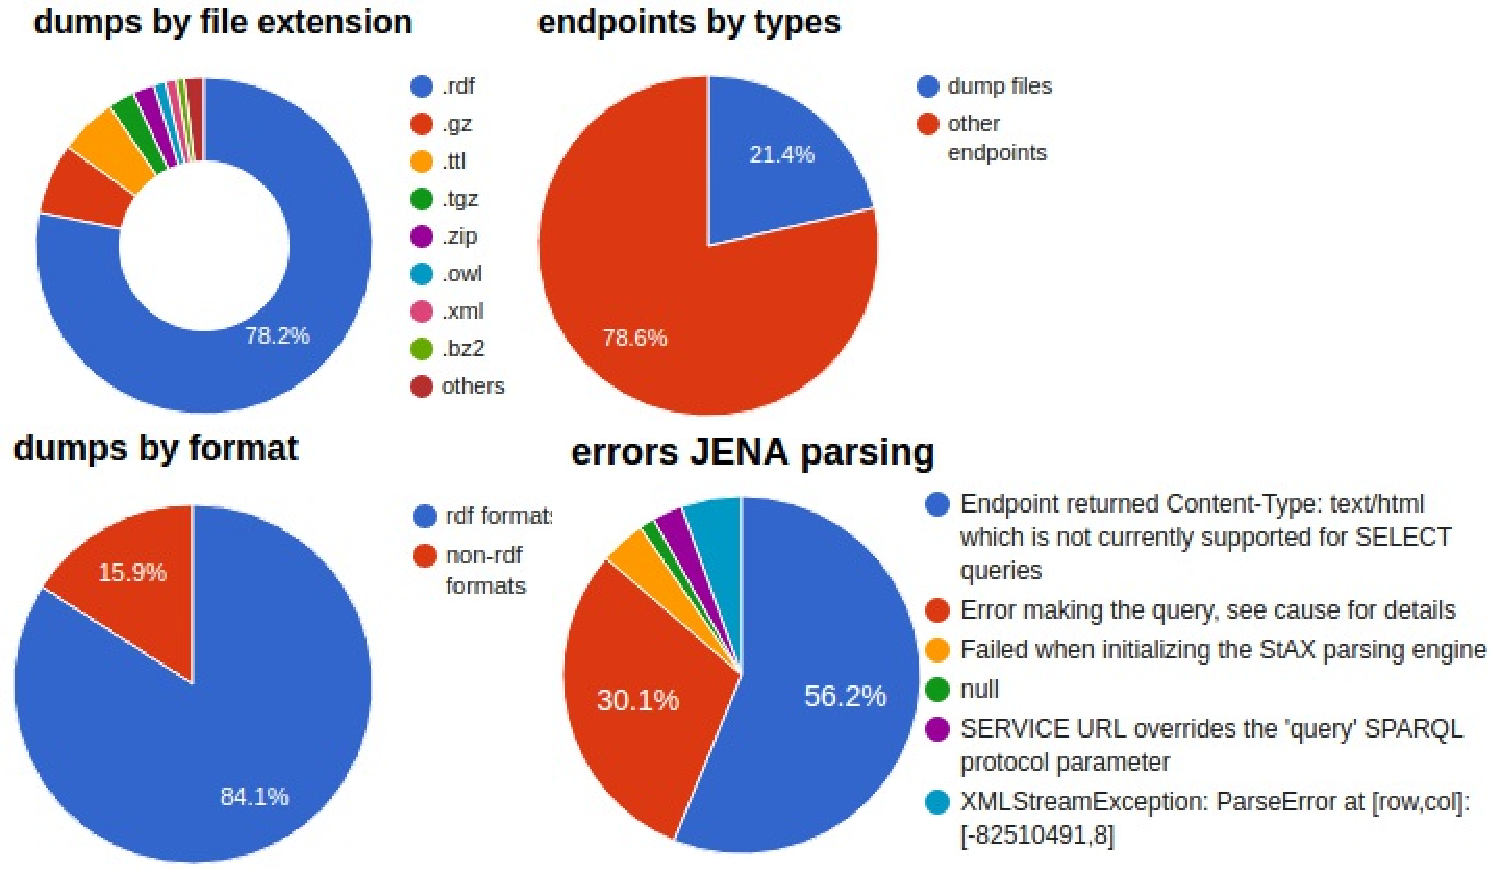
\includegraphics[width=340pt]{img/dumps3.pdf}
	\caption{Dump files and Apache Jena parsing error.}
	\label{fig:dumps}
\end{figure}

Finally, we validated our heuristic assessing if the URI really belongs to the dataset with more literals.
To this end, we took a sample of 100 URIs\footnote{Link to the sample data: \url{https://github.com/dice-group/wimu/blob/master/result100.csv}} that belong to at least two datasets, where we assess manually the data in order to check if the results are really correct. 
As a result, the dataset containing the correct information was found as first result in 90\% of the URIs and among the top three in 95\% of the URIs.

%\section{Conclusion and Future work}

